\documentclass[../master/master.tex]{subfiles}

\begin{document}

%----------------------------------------------------------------------
% LECTURE 13: The Riemann Integral
% Date: March 17, 2026
%----------------------------------------------------------------------
\renewcommand{\lecturenum}{13}
\renewcommand{\lecturedate}{March 17, 2026}
\renewcommand{\lecturetopic}{The Riemann Integral}

\section{Lecture \lecturenum : \lecturedate}

\begin{lecturesummary}
\textbf{Lecture Overview:} We introduce the Riemann integral via the machinery of partitions, upper sums, and lower sums. A partition of $[a,b]$ splits the interval into finitely many subintervals; on each one we take the supremum and infimum of a bounded function $f$ to form upper and lower Darboux sums $U(P,f)$ and $L(P,f)$. Taking the infimum over all partitions gives the upper Riemann integral $\overline{\int}$, and the supremum gives the lower Riemann integral $\underline{\int}$. When these two agree, $f$ is Riemann integrable.
\end{lecturesummary}

\subsection{Partitions and Darboux Sums}

\begin{summarybox}
\textbf{Section Overview:} We define partitions of a closed interval $[a,b]$, the associated quantities $\Delta x_i$, $M_i$, $m_i$, and build the upper and lower Darboux sums $U(P,f)$ and $L(P,f)$ that bound the ``area under the curve'' from above and below.
\end{summarybox}

\begin{definition}
A \defn{partition} of $[a,b]$ is a finite set of points $P = \{x_0, x_1, \dots, x_n\}$ such that
\[
a = x_0 \leq x_1 \leq \cdots \leq x_n = b.
\]
\end{definition}

\begin{definition}
Given a partition $P = \{x_0, x_1, \dots, x_n\}$ of $[a,b]$ and a bounded function $f: [a,b] \to \R$, define for each $i = 1, 2, \dots, n$:
\begin{align*}
\Delta x_i &= x_i - x_{i-1}, \\
M_i &= \sup_{x \in [x_{i-1}, x_i]} f(x), \\
m_i &= \inf_{x \in [x_{i-1}, x_i]} f(x).
\end{align*}
The \defn{upper Darboux sum} of $f$ with respect to $P$ is
\[
U(P, f) = \sum_{i=1}^{n} M_i \, \Delta x_i,
\]
and the \defn{lower Darboux sum} of $f$ with respect to $P$ is
\[
L(P, f) = \sum_{i=1}^{n} m_i \, \Delta x_i.
\]
\end{definition}

\begin{remark}
Since $m_i \leq M_i$ for all $i$, we always have $L(P,f) \leq U(P,f)$ for any partition $P$.
\end{remark}

\subsection{Upper and Lower Riemann Integrals}

\begin{summarybox}
\textbf{Section Overview:} By taking the infimum of all upper sums and the supremum of all lower sums, we obtain the upper and lower Riemann integrals. When these coincide, $f$ is Riemann integrable on $[a,b]$.
\end{summarybox}

\begin{definition}
Let $f: [a,b] \to \R$ be bounded. The \defn{upper Riemann integral} of $f$ over $[a,b]$ is
\[
\overline{\int_a^b} f \, dx = \inf_P \, U(P, f),
\]
and the \defn{lower Riemann integral} of $f$ over $[a,b]$ is
\[
\underline{\int_a^b} f \, dx = \sup_P \, L(P, f),
\]
where the infimum and supremum are taken over all partitions $P$ of $[a,b]$.
\end{definition}

\begin{definition}
A bounded function $f: [a,b] \to \R$ is \defn{Riemann integrable} on $[a,b]$, written $f \in \mathscr{R}$ on $[a,b]$, if
\[
\overline{\int_a^b} f \, dx = \underline{\int_a^b} f \, dx.
\]
In this case, the common value is called the \defn{Riemann integral} of $f$ and is denoted
\[
\int_a^b f \, dx.
\]
\end{definition}

\begin{definition}
A \defn{measure} on a set $X$ is a function $\mu: 2^X \to \R$ such that
\begin{enumerate}[label=(\roman*)]
    \item $\mu(\emptyset) = 0$,
    \item $\mu(E) \geq 0$ for all $E \subseteq X$,
    \item If $E_1, E_2, \dots$ are pairwise disjoint, then $\displaystyle\mu\!\left(\bigcup_{i=1}^{\infty} E_i\right) = \sum_{i=1}^{\infty} \mu(E_i)$.
\end{enumerate}
\end{definition}

\begin{example}
Examples of measures:
\begin{enumerate}[label=(\roman*)]
    \item The \defn{Lebesgue measure} on $\R$ assigns to each interval its length: $\mu([a,b]) = b - a$.
    \item The \defn{counting measure} (discrete measure): $\mu(E) = |E|$, the number of elements in $E$.
    \item The \defn{Haar measure} on a group: a measure that is invariant under the group operation.
    \item A \defn{probability measure} (distribution): a measure with $\mu(X) = 1$.
    \item The \defn{Dirac measure} at a point $x_0$: $\mu(E) = \begin{cases} 1 & \text{if } x_0 \in E, \\ 0 & \text{if } x_0 \notin E. \end{cases}$
\end{enumerate}
\end{example}

\begin{theorem}
The Riemann integral $\int_a^b f \, dx$ exists (i.e., $f \in \mathscr{R}$ on $[a,b]$) in each of the following cases:
\begin{enumerate}[label=(\roman*)]
    \item $f$ is continuous on $[a,b]$,
    \item $f$ is monotonic on $[a,b]$,
    \item $f$ is bounded on $[a,b]$ with finitely many discontinuities,
    \item $f \circ g$ where $g \in \mathscr{R}$ on $[a,b]$.
\end{enumerate}
\end{theorem}

\begin{definition}
Let $P$ be a partition of $[a,b]$. A partition $P^*$ is a \defn{refinement} of $P$ if $P \subseteq P^*$.
\end{definition}

\begin{theorem}
If $P^*$ is a refinement of $P$, then
\[
L(P, f) \leq L(P^*, f) \leq U(P^*, f) \leq U(P, f).
\]
\end{theorem}

\begin{proof}
By induction on $|P^* \setminus P|$.

\textbf{Base case:} $P^* \setminus P = \{x\}$, a single point, where $x_{i-1} \leq x \leq x_i$ for some $i$.

\begin{center}
\begin{tikzpicture}[scale=1.2]
    % Axes
    \draw[->] (-0.3,0) -- (5.5,0) node[right] {};
    \draw[->] (0,-0.3) -- (0,3.5) node[above] {};

    % Curve (only on [x_{i-1}, x_i])
    \draw[thick, blue, domain=1:4.5, smooth, samples=50]
        plot (\x, {0.3*(\x-1.5)*(\x-3.5)*(\x-4.5) + 2});

    % Partition points
    \draw[thick] (1,0.05) -- (1,-0.05) node[below] {$x_{i-1}$};
    \draw[thick] (4.5,0.05) -- (4.5,-0.05) node[below] {$x_i$};
    \draw[thick, red] (2.8,0.05) -- (2.8,-0.05) node[below] {\color{red}$x$};

    % Dashed vertical lines
    \draw[dashed, gray] (1,0) -- (1,2.63);
    \draw[dashed, gray] (4.5,0) -- (4.5,2.63);
    \draw[dashed, red] (2.8,0) -- (2.8,2.63);

    % M_i line (sup)
    \draw[thick, green!50!black, dashed] (1,2.63) -- (4.5,2.63) node[right] {$M_i = \sup f$};

    % m_i line (inf)
    \draw[thick, orange!70!black, dashed] (1,0.69) -- (4.5,0.69) node[right] {$m_i = \inf f$};
\end{tikzpicture}
\end{center}

Adding the single point $x$ splits the interval $[x_{i-1}, x_i]$ into $[x_{i-1}, x]$ and $[x, x_i]$. Let
\begin{align*}
w_1 &= \inf_{t \in [x_{i-1}, x]} f(t), \quad W_1 = \sup_{t \in [x_{i-1}, x]} f(t), \\
w_2 &= \inf_{t \in [x, x_i]} f(t), \quad W_2 = \sup_{t \in [x, x_i]} f(t).
\end{align*}
Since $[x_{i-1}, x] \subseteq [x_{i-1}, x_i]$ and $[x, x_i] \subseteq [x_{i-1}, x_i]$, we have
\[
m_i \leq w_1, \quad m_i \leq w_2, \quad W_1 \leq M_i, \quad W_2 \leq M_i.
\]
Now the lower sum changes only in the $i$-th term:
\begin{align*}
L(P^*, f) - L(P, f) &= w_1(x - x_{i-1}) + w_2(x_i - x) - m_i(x_i - x_{i-1}) \\
&\geq m_i(x - x_{i-1}) + m_i(x_i - x) - m_i(x_i - x_{i-1}) = 0.
\end{align*}
So $L(P, f) \leq L(P^*, f)$. Similarly,
\begin{align*}
U(P, f) - U(P^*, f) &= M_i(x_i - x_{i-1}) - W_1(x - x_{i-1}) - W_2(x_i - x) \\
&\geq M_i(x_i - x_{i-1}) - M_i(x - x_{i-1}) - M_i(x_i - x) = 0.
\end{align*}
So $U(P^*, f) \leq U(P, f)$. The inequality $L(P^*, f) \leq U(P^*, f)$ is immediate, giving
\[
L(P, f) \leq L(P^*, f) \leq U(P^*, f) \leq U(P, f).
\]

\textbf{Inductive step:} If $|P^* \setminus P| = k$, pick any $x \in P^* \setminus P$ and let $P' = P \cup \{x\}$. Then $|P^* \setminus P'| = k - 1$, so by the inductive hypothesis
\[
L(P', f) \leq L(P^*, f) \leq U(P^*, f) \leq U(P', f),
\]
and by the base case
\[
L(P, f) \leq L(P', f) \quad \text{and} \quad U(P', f) \leq U(P, f).
\]
Combining gives the result.
\end{proof}

\begin{remark}
One might ask: can we induct on uncountably infinite sets? Ordinary induction only applies to $\N$, so it handles finite steps. This is not an issue here, since partitions are finite sets by definition, and $|P^* \setminus P| \in \N$. For uncountable settings, there is a more powerful tool called \defn{transfinite induction} (induction over ordinals), but this belongs to set theory and is beyond the scope of this course.
\end{remark}

\begin{notebox}
\textbf{Technique: Induction on set difference.} When you need to show a property holds for a refinement $P^* \supseteq P$, induct on $|P^* \setminus P|$, the number of added points. The base case handles adding a single point --- this is where the real work happens, and it typically reduces to comparing quantities on one interval versus its two sub-intervals. The inductive step is then essentially free: add one point at a time, apply the base case, and chain the inequalities. This ``one point at a time'' strategy appears whenever you refine a partition, mesh, or discretization.
\end{notebox}

\begin{theorem}
For any bounded function $f$ on $[a,b]$,
\[
\sup_P L(P, f) \leq \inf_P U(P, f).
\]
That is, $\underline{\int_a^b} f\, dx \leq \overline{\int_a^b} f\, dx$.
\end{theorem}

\begin{proof}
Let $P_1$ and $P_2$ be any two partitions of $[a,b]$. Then $P_1 \cup P_2$ is a refinement of both, so by the previous theorem:
\[
L(P_1, f) \leq L(P_1 \cup P_2, f) \leq U(P_1 \cup P_2, f) \leq U(P_2, f).
\]
Thus $L(P_1, f) \leq U(P_2, f)$ for all partitions $P_1, P_2$. Since $L(P_1, f) \leq U(P_2, f)$ holds for every $P_2$, we have $L(P_1, f) \leq \inf_{P_2} U(P_2, f)$ for every $P_1$. Taking the supremum over $P_1$:
\[
\sup_{P_1} L(P_1, f) \leq \inf_{P_2} U(P_2, f). \qedhere
\]
\end{proof}

\begin{theorem}
A bounded function $f$ is Riemann integrable on $[a,b]$ if and only if for every $\eps > 0$, there exists a partition $P$ of $[a,b]$ such that
\[
U(P, f) - L(P, f) < \eps.
\]
\end{theorem}

\begin{proof}
$(\Rightarrow)$ Suppose $f \in \mathscr{R}$ on $[a,b]$, so $\underline{\int_a^b} f\,dx = \overline{\int_a^b} f\,dx = \int_a^b f\,dx$. Let $\eps > 0$. Since $\int_a^b f\,dx = \sup_P L(P,f)$, there exists a partition $P_1$ such that
\[
\int_a^b f\,dx - L(P_1, f) < \frac{\eps}{2}.
\]
Since $\int_a^b f\,dx = \inf_P U(P,f)$, there exists a partition $P_2$ such that
\[
U(P_2, f) - \int_a^b f\,dx < \frac{\eps}{2}.
\]
Let $P = P_1 \cup P_2$. Since $P$ refines both $P_1$ and $P_2$:
\[
U(P, f) - L(P, f) \leq U(P_2, f) - L(P_1, f) = \left(U(P_2, f) - \int_a^b f\,dx\right) + \left(\int_a^b f\,dx - L(P_1, f)\right) < \frac{\eps}{2} + \frac{\eps}{2} = \eps.
\]

$(\Leftarrow)$ Suppose for every $\eps > 0$ there exists $P$ with $U(P,f) - L(P,f) < \eps$. Since $L(P,f) \leq \underline{\int} \leq \overline{\int} \leq U(P,f)$, we have
\[
0 \leq \overline{\int_a^b} f\,dx - \underline{\int_a^b} f\,dx \leq U(P,f) - L(P,f) < \eps.
\]
Since this holds for all $\eps > 0$, we conclude $\overline{\int_a^b} f\,dx = \underline{\int_a^b} f\,dx$, so $f \in \mathscr{R}$.
\end{proof}

\begin{theorem}
If $P = \{x_0, x_1, \dots, x_n\}$ is a partition of $[a,b]$ such that $U(P,f) - L(P,f) < \eps$ and $f \in \mathscr{R}$ on $[a,b]$, then for any choice of sample points $t_i \in [x_{i-1}, x_i]$,
\[
\left| \sum_{i=1}^{n} f(t_i) \, \Delta x_i - \int_a^b f \, dx \right| < \eps.
\]
\end{theorem}

\begin{proof}
Since $m_i \leq f(t_i) \leq M_i$ for each $i$, we have
\[
L(P, f) = \sum_{i=1}^{n} m_i \, \Delta x_i \leq \sum_{i=1}^{n} f(t_i) \, \Delta x_i \leq \sum_{i=1}^{n} M_i \, \Delta x_i = U(P, f).
\]
Also, $L(P, f) \leq \int_a^b f\,dx \leq U(P, f)$. Both the Riemann sum and the integral lie in the interval $[L(P,f),\, U(P,f)]$, which has length less than $\eps$, so
\[
\left| \sum_{i=1}^{n} f(t_i) \, \Delta x_i - \int_a^b f \, dx \right| \leq U(P,f) - L(P,f) < \eps. \qedhere
\]
\end{proof}

\begin{theorem}
If $f$ is continuous on $[a,b]$, then $f \in \mathscr{R}$ on $[a,b]$.
\end{theorem}

\begin{proof}
Let $\eps > 0$. Since $f$ is continuous on the compact set $[a,b]$, $f$ is uniformly continuous. Thus there exists $\delta > 0$ such that for all $x, t \in [a,b]$,
\[
|x - t| < \delta \implies |f(x) - f(t)| < \frac{\eps}{b - a}.
\]
Let $P = \{x_0, x_1, \dots, x_n\}$ be any partition of $[a,b]$ with $\Delta x_i < \delta$ for all $i$. Then on each subinterval $[x_{i-1}, x_i]$, any two points are within $\delta$ of each other, so
\[
M_i - m_i < \frac{\eps}{b - a}.
\]
Therefore
\[
U(P, f) - L(P, f) = \sum_{i=1}^{n} (M_i - m_i) \, \Delta x_i < \frac{\eps}{b - a} \sum_{i=1}^{n} \Delta x_i = \frac{\eps}{b - a} \cdot (b - a) = \eps.
\]
By the previous theorem, $f \in \mathscr{R}$ on $[a,b]$.
\end{proof}

\begin{theorem}
If $f$ is monotonic on $[a,b]$, then $f \in \mathscr{R}$ on $[a,b]$.
\end{theorem}

\begin{proof}
Without loss of generality, assume $f$ is monotonically increasing (the decreasing case is analogous). Then on each subinterval $[x_{i-1}, x_i]$,
\[
m_i = f(x_{i-1}), \quad M_i = f(x_i).
\]
Let $\eps > 0$. Choose the uniform partition $P = \{x_0, x_1, \dots, x_n\}$ with $\Delta x_i = \frac{b-a}{n}$ for all $i$, where $n$ is large enough that $\frac{(b-a)}{n}(f(b) - f(a)) < \eps$. Then
\[
U(P,f) - L(P,f) = \sum_{i=1}^{n} (M_i - m_i)\,\Delta x_i = \frac{b-a}{n} \sum_{i=1}^{n} \bigl(f(x_i) - f(x_{i-1})\bigr) = \frac{b-a}{n}\bigl(f(b) - f(a)\bigr) < \eps.
\]
The sum telescopes, leaving only $f(b) - f(a)$. By the previous characterization, $f \in \mathscr{R}$ on $[a,b]$.
\end{proof}

\begin{example}
Define $f: [0,1] \to \R$ by
\[
f(x) = \begin{cases} \dfrac{1}{q} & \text{if } x = \dfrac{p}{q} \in \Q \text{ in lowest terms}, \\[6pt] 0 & \text{if } x \notin \Q. \end{cases}
\]
\end{example}

\begin{center}
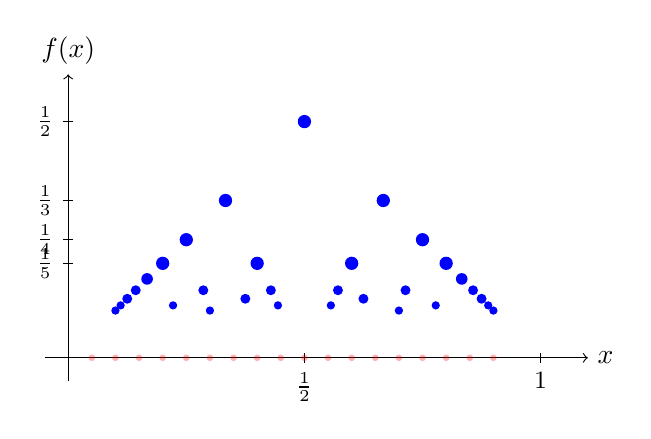
\begin{tikzpicture}[scale=6]
    % Axes
    \draw[->] (-0.05,0) -- (1.1,0) node[right] {$x$};
    \draw[->] (0,-0.05) -- (0,0.6) node[above] {$f(x)$};

    % Tick marks on x-axis
    \draw (1,0.01) -- (1,-0.01) node[below] {\small $1$};
    \draw (0.5,0.01) -- (0.5,-0.01) node[below] {\small $\frac{1}{2}$};

    % Tick marks on y-axis
    \draw (0.01,0.5) -- (-0.01,0.5) node[left] {\small $\frac{1}{2}$};
    \draw (0.01,0.333) -- (-0.01,0.333) node[left] {\small $\frac{1}{3}$};
    \draw (0.01,0.25) -- (-0.01,0.25) node[left] {\small $\frac{1}{4}$};
    \draw (0.01,0.2) -- (-0.01,0.2) node[left] {\small $\frac{1}{5}$};

    % q=2: 1/2
    \fill[blue] (0.5,0.5) circle (0.4pt);

    % q=3: 1/3, 2/3
    \fill[blue] (0.333,0.333) circle (0.4pt);
    \fill[blue] (0.667,0.333) circle (0.4pt);

    % q=4: 1/4, 3/4
    \fill[blue] (0.25,0.25) circle (0.4pt);
    \fill[blue] (0.75,0.25) circle (0.4pt);

    % q=5: 1/5, 2/5, 3/5, 4/5
    \fill[blue] (0.2,0.2) circle (0.4pt);
    \fill[blue] (0.4,0.2) circle (0.4pt);
    \fill[blue] (0.6,0.2) circle (0.4pt);
    \fill[blue] (0.8,0.2) circle (0.4pt);

    % q=6: 1/6, 5/6
    \fill[blue] (0.167,0.167) circle (0.35pt);
    \fill[blue] (0.833,0.167) circle (0.35pt);

    % q=7: 1/7, 2/7, 3/7, 4/7, 5/7, 6/7
    \fill[blue] (0.143,0.143) circle (0.3pt);
    \fill[blue] (0.286,0.143) circle (0.3pt);
    \fill[blue] (0.429,0.143) circle (0.3pt);
    \fill[blue] (0.571,0.143) circle (0.3pt);
    \fill[blue] (0.714,0.143) circle (0.3pt);
    \fill[blue] (0.857,0.143) circle (0.3pt);

    % q=8: 1/8, 3/8, 5/8, 7/8
    \fill[blue] (0.125,0.125) circle (0.3pt);
    \fill[blue] (0.375,0.125) circle (0.3pt);
    \fill[blue] (0.625,0.125) circle (0.3pt);
    \fill[blue] (0.875,0.125) circle (0.3pt);

    % q=9: 1/9, 2/9, 4/9, 5/9, 7/9, 8/9
    \fill[blue] (0.111,0.111) circle (0.25pt);
    \fill[blue] (0.222,0.111) circle (0.25pt);
    \fill[blue] (0.444,0.111) circle (0.25pt);
    \fill[blue] (0.556,0.111) circle (0.25pt);
    \fill[blue] (0.778,0.111) circle (0.25pt);
    \fill[blue] (0.889,0.111) circle (0.25pt);

    % q=10: 1/10, 3/10, 7/10, 9/10
    \fill[blue] (0.1,0.1) circle (0.25pt);
    \fill[blue] (0.3,0.1) circle (0.25pt);
    \fill[blue] (0.7,0.1) circle (0.25pt);
    \fill[blue] (0.9,0.1) circle (0.25pt);

    % Irrational points along x-axis (f=0)
    \foreach \x in {0.05,0.1,...,0.95} {
        \fill[red, opacity=0.3] (\x,0) circle (0.2pt);
    }
\end{tikzpicture}
\end{center}

\noindent Is $f$ Riemann integrable? Yes! Note that $L(P,f) = 0$ for every partition $P$, since every subinterval contains irrationals. The key observation is that for any $\eps > 0$, only finitely many rationals $p/q$ in $[0,1]$ satisfy $1/q \geq \eps$, so we can trap them in subintervals of arbitrarily small total length, making $U(P,f)$ arbitrarily close to $0$. Thus $\int_0^1 f\,dx = 0$.

\begin{theorem}
If $f$ is bounded on $[a,b]$ and $f$ has only finitely many points of discontinuity, then $f \in \mathscr{R}$ on $[a,b]$.
\end{theorem}

\begin{proof}
Let $E = \{e_1, \dots, e_m\}$ be the set of discontinuities of $f$. Cover $E$ by finitely many disjoint open intervals $(u_j, v_j)$ such that for every $e \in E$, $e \in (u_j, v_j)$ for some $j$. The complement
\[
K = [a,b] \setminus \bigcup_{j=1}^{m} (u_j, v_j)
\]
is compact. Since $f$ is bounded, let $M$ be such that $|f(x)| \leq M$ for all $x \in [a,b]$. Then on any subinterval, $M_i - m_i \leq 2M$.

Let $\eps > 0$. Choose $\delta < \dfrac{\eps}{4M}$. Cover $E$ with intervals $[u_j, v_j]$ such that
\[
\sum_{j=1}^{m} (v_j - u_j) < \delta.
\]
On the compact set $K = [a,b] \setminus \bigcup_j (u_j, v_j)$, $f$ is continuous, hence uniformly continuous. Choose a partition $P$ fine enough that on each subinterval of $P$ lying in $K$, we have $M_i - m_i < \dfrac{\eps}{2(b-a)}$. Include the points $u_j, v_j$ in $P$. Then
\[
U(P,f) - L(P,f) = \underbrace{\sum_{\substack{i \\ [x_{i-1},x_i] \subseteq K}} (M_i - m_i)\,\Delta x_i}_{< \,\frac{\eps}{2(b-a)} \cdot (b-a) \,=\, \eps/2} + \underbrace{\sum_{\substack{i \\ [x_{i-1},x_i] \subseteq [u_j,v_j]}} (M_i - m_i)\,\Delta x_i}_{\leq \,2M \cdot \delta \,<\, \eps/2} < \frac{\eps}{2} + \frac{\eps}{2} = \eps.
\]
Thus $f \in \mathscr{R}$ on $[a,b]$.
\end{proof}

\begin{theorem}
Suppose $f \in \mathscr{R}$ on $[a,b]$ with $m \leq f(x) \leq M$ for all $x \in [a,b]$, and $g$ is continuous on $[m, M]$. Then $h = g \circ f$ is Riemann integrable on $[a,b]$.
\end{theorem}

\begin{proof}
Let $\eps > 0$. Since $g$ is continuous on the compact set $[m, M]$, it is uniformly continuous: there exists $\delta > 0$ such that
\[
|s - t| < \delta \implies |g(s) - g(t)| < \eps.
\]
We may assume $\delta < \eps$. Since $f \in \mathscr{R}$, choose a partition $P = \{x_0, \dots, x_n\}$ such that $U(P, f) - L(P, f) < \delta^2$. Let
\[
M_i^f = \sup_{[x_{i-1},x_i]} f, \quad m_i^f = \inf_{[x_{i-1},x_i]} f, \quad M_i^h = \sup_{[x_{i-1},x_i]} h, \quad m_i^h = \inf_{[x_{i-1},x_i]} h.
\]
Partition the indices $\{1, \dots, n\}$ into two sets:
\begin{align*}
A &= \{i : M_i^f - m_i^f < \delta\}, \\
B &= \{i : M_i^f - m_i^f \geq \delta\}.
\end{align*}
For $i \in A$: the oscillation of $f$ on $[x_{i-1}, x_i]$ is less than $\delta$, so by uniform continuity of $g$, $M_i^h - m_i^h < \eps$.

For $i \in B$: since $g$ is continuous on the compact set $[m,M]$, $g$ is bounded, say $|g| \leq K$. Then $M_i^h - m_i^h \leq 2K$. Also,
\[
\delta \sum_{i \in B} \Delta x_i \leq \sum_{i \in B} (M_i^f - m_i^f)\,\Delta x_i \leq U(P,f) - L(P,f) < \delta^2,
\]
so $\sum_{i \in B} \Delta x_i < \delta$.

Combining:
\[
U(P, h) - L(P, h) = \sum_{i \in A} (M_i^h - m_i^h)\,\Delta x_i + \sum_{i \in B} (M_i^h - m_i^h)\,\Delta x_i < \eps(b - a) + 2K\delta < \eps(b - a) + 2K\eps.
\]
Since $\eps$ is arbitrary, $h \in \mathscr{R}$ on $[a,b]$.
\end{proof}

\begin{example}[Zeno Staircase]
Define $f: [0,1] \to \R$ by
\[
f(x) = \frac{k}{2^n} \quad \text{for } x \in \left[\frac{k}{2^n}, \frac{k+1}{2^n}\right), \quad \text{i.e., } f = \sum_{n=1}^{\infty} \frac{1}{2^n} \mathbf{1}_{[1-1/2^n,\, 1)}.
\]
Equivalently, $f$ jumps by $1/2^n$ at $x = 1 - 1/2^n$:

\begin{center}
\begin{tikzpicture}[scale=5]
    % Axes
    \draw[->] (-0.05,0) -- (1.15,0) node[right] {$x$};
    \draw[->] (0,-0.05) -- (0,1.15) node[above] {$f(x)$};

    % Tick marks
    \draw (1,0.01) -- (1,-0.01) node[below] {\small $1$};
    \draw (0.01,1) -- (-0.01,1) node[left] {\small $1$};

    % Step 0: [0, 1/2) at height 0
    \draw[thick, blue] (0,0) -- (0.5,0);

    % Step 1: [1/2, 3/4) at height 1/2
    \draw[thick, blue] (0.5,0.5) -- (0.75,0.5);
    \fill[blue] (0.5,0.5) circle (0.4pt);
    \draw[blue, fill=white] (0.5,0) circle (0.4pt);
    \node[below] at (0.5,-0.01) {\small $\frac{1}{2}$};
    \node[left] at (-0.01,0.5) {\small $\frac{1}{2}$};

    % Step 2: [3/4, 7/8) at height 3/4
    \draw[thick, blue] (0.75,0.75) -- (0.875,0.75);
    \fill[blue] (0.75,0.75) circle (0.4pt);
    \draw[blue, fill=white] (0.75,0.5) circle (0.4pt);
    \node[below] at (0.75,-0.01) {\small $\frac{3}{4}$};
    \node[left] at (-0.01,0.75) {\small $\frac{3}{4}$};

    % Step 3: [7/8, 15/16) at height 7/8
    \draw[thick, blue] (0.875,0.875) -- (0.9375,0.875);
    \fill[blue] (0.875,0.875) circle (0.4pt);
    \draw[blue, fill=white] (0.875,0.75) circle (0.4pt);
    \node[below] at (0.875,-0.01) {\small $\frac{7}{8}$};
    \node[left] at (-0.01,0.875) {\small $\frac{7}{8}$};

    % Step 4: [15/16, 31/32) at height 15/16
    \draw[thick, blue] (0.9375,0.9375) -- (0.96875,0.9375);
    \fill[blue] (0.9375,0.9375) circle (0.3pt);
    \draw[blue, fill=white] (0.9375,0.875) circle (0.3pt);

    % Step 5
    \draw[thick, blue] (0.96875,0.96875) -- (0.984375,0.96875);
    \fill[blue] (0.96875,0.96875) circle (0.25pt);
    \draw[blue, fill=white] (0.96875,0.9375) circle (0.25pt);

    % Dots suggesting continuation
    \node at (0.995,0.995) {\small $\cdots$};

    % f(1) = 1
    \fill[blue] (1,1) circle (0.4pt);

    % Dashed line to 1
    \draw[dashed, gray] (1,0) -- (1,1);
    \draw[dashed, gray] (0,1) -- (1,1);
\end{tikzpicture}
\end{center}

This function is bounded, monotonically increasing, and has countably many discontinuities (at $x = 1 - 1/2^n$ for $n = 1, 2, \dots$). By the previous theorems, $f \in \mathscr{R}$ on $[0,1]$. Note that $f$ has infinitely many discontinuities, so the finite-discontinuity theorem does not apply directly. However, $f$ is monotonically increasing, which guarantees integrability.
\end{example}

\end{document}
